

\documentclass{report}
\usepackage{graphicx}
\title{Caveau\_1566}
\author{Ding Jérémy}
\date{\today}

\begin{document}

\maketitle
\tableofcontents
\section{Introduction}

This project consists of the realization of an LED panel that displays
the text ``Caveau''. It is intended to be used at parties and mounted
on a wall.

\section{Specifications}

The panel must meet the following requirements:

\begin{itemize}
    \item Must operate from a 230 VAC power supply.
    \item Must be visible during both daytime and nighttime.
    \item Must display the text ``Caveau''.
\end{itemize}

\section{Design}
In this section, the design of the panel is chosen.
\subsection{Sketch}
First, a sketch is drawn, the idea here is to place the main elements as well as define the main dimensions.

\begin{figure}[htbp]
    \centering
    \includegraphics[width=0.8\textwidth]{figures/schema\_mecanique.drawio.png}
    \caption{Front view}
    \label{fig:front-view}
\end{figure}

The figure~\ref{fig:front-view} shows the text ``Caveau'' with an
arrow. It also includes a logo representing the company's emblem.
This figure shows the front view of the panel.

\begin{figure}[htbp]
    \centering
    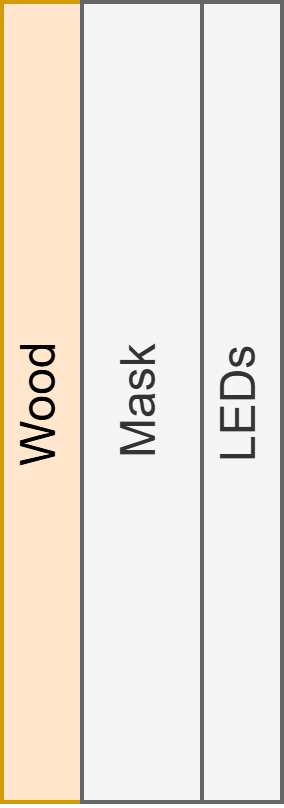
\includegraphics[width=0.2\textwidth]{figures/layers.drawio.png}
    \caption{Side view}
    \label{fig:layers}
\end{figure}

The idea is to have three distinct layers.

\begin{enumerate}
    \item A thin layer of wood capable of letting light through.
    \item A mask layer, 3D printed, which serves to focus the light
    into the desired shape.
    \item A LED layer consisting of a simple plane where the LEDs are
    mounted in a pattern matching the mask.
\end{enumerate}

\end{document}